\documentclass{beamer}
\usepackage[utf8]{inputenc}
\usepackage{url}
\usepackage{hyperref}
\graphicspath{{./fig/aula4}}

\usepackage{color}
\definecolor{lightgray}{rgb}{0.95, 0.95, 0.95}
\definecolor{darkgray}{rgb}{0.4, 0.4, 0.4}
%\definecolor{purple}{rgb}{0.65, 0.12, 0.82}
\definecolor{editorGray}{rgb}{0.95, 0.95, 0.95}
\definecolor{editorOcher}{rgb}{1, 0.5, 0} % #FF7F00 -> rgb(239, 169, 0)
\definecolor{editorGreen}{rgb}{0, 0.5, 0} % #007C00 -> rgb(0, 124, 0)
\definecolor{orange}{rgb}{1,0.45,0.13}		
\definecolor{olive}{rgb}{0.17,0.59,0.20}
\definecolor{brown}{rgb}{0.69,0.31,0.31}
\definecolor{purple}{rgb}{0.38,0.18,0.81}
\definecolor{lightblue}{rgb}{0.1,0.57,0.7}
\definecolor{lightred}{rgb}{1,0.4,0.5}
\usepackage{upquote}
\usepackage{listings}
% CSS
\lstdefinelanguage{CSS}{
  keywords={color,background-image:,margin,padding,font,weight,display,position,top,left,right,bottom,list,style,border,size,white,space,min,width, transition:, transform:, transition-property, transition-duration, transition-timing-function},	
  sensitive=true,
  morecomment=[l]{//},
  morecomment=[s]{/*}{*/},
  morestring=[b]',
  morestring=[b]",
  alsoletter={:},
  alsodigit={-}
}

% JavaScript
\lstdefinelanguage{JavaScript}{
  morekeywords={typeof, new, true, false, catch, function, return, null, catch, switch, var, if, in, while, do, else, case, break},
  morecomment=[s]{/*}{*/},
  morecomment=[l]//,
  morestring=[b]",
  morestring=[b]'
}

\lstdefinelanguage{HTML5}{
  language=html,
  sensitive=true,	
  alsoletter={<>=-},	
  morecomment=[s]{<!-}{-->},
  tag=[s],
  otherkeywords={
  % General
  >,
  % Standard tags
	<!DOCTYPE,
  </html, <html, <head, <title, </title, <style, </style, <link, </head, <meta, />,
	% body
	</body, <body,
	% Divs
	</div, <div, </div>, 
	% Paragraphs
	</p, <p, </p>,
	% scripts
	</script, <script,
  % More tags...
  <canvas, /canvas>, <svg, <rect, <animateTransform, </rect>, </svg>, <video, <source, <iframe, </iframe>, </video>, <image, </image>, <header, </header, <article, </article
  },
  ndkeywords={
  % General
  =,
  % HTML attributes
  charset=, src=, id=, width=, height=, style=, type=, rel=, href=,
  % SVG attributes
  fill=, attributeName=, begin=, dur=, from=, to=, poster=, controls=, x=, y=, repeatCount=, xlink:href=,
  % properties
  margin:, padding:, background-image:, border:, top:, left:, position:, width:, height:, margin-top:, margin-bottom:, font-size:, line-height:,
	% CSS3 properties
  transform:, -moz-transform:, -webkit-transform:,
  animation:, -webkit-animation:,
  transition:,  transition-duration:, transition-property:, transition-timing-function:,
  }
}

\lstdefinestyle{htmlcssjs} {%
  % General design
%  backgroundcolor=\color{editorGray},
  basicstyle={\footnotesize\ttfamily},   
  frame=b,
  % line-numbers
  xleftmargin={0.75cm},
  numbers=left,
  stepnumber=1,
  firstnumber=1,
  numberfirstline=true,	
  % Code design
  identifierstyle=\color{black},
  keywordstyle=\color{blue}\bfseries,
  ndkeywordstyle=\color{editorGreen}\bfseries,
  stringstyle=\color{editorOcher}\ttfamily,
  commentstyle=\color{brown}\ttfamily,
  % Code
  language=HTML5,
  alsolanguage=JavaScript,
  alsodigit={.:;},	
  tabsize=2,
  showtabs=false,
  showspaces=false,
  showstringspaces=false,
  extendedchars=true,
  breaklines=true,
  % German umlauts
  literate=%
  {Ö}{{\"O}}1
  {Ä}{{\"A}}1
  {Ü}{{\"U}}1
  {ß}{{\ss}}1
  {ü}{{\"u}}1
  {ä}{{\"a}}1
  {ö}{{\"o}}1
}
%
\lstdefinestyle{py} {%
language=python,
literate=%
*{0}{{{\color{lightred}0}}}1
{1}{{{\color{lightred}1}}}1
{2}{{{\color{lightred}2}}}1
{3}{{{\color{lightred}3}}}1
{4}{{{\color{lightred}4}}}1
{5}{{{\color{lightred}5}}}1
{6}{{{\color{lightred}6}}}1
{7}{{{\color{lightred}7}}}1
{8}{{{\color{lightred}8}}}1
{9}{{{\color{lightred}9}}}1,
basicstyle=\footnotesize\ttfamily, % Standardschrift
numbers=left,               % Ort der Zeilennummern
%numberstyle=\tiny,          % Stil der Zeilennummern
%stepnumber=2,               % Abstand zwischen den Zeilennummern
numbersep=5pt,              % Abstand der Nummern zum Text
tabsize=4,                  % Groesse von Tabs
extendedchars=true,         %
breaklines=true,            % Zeilen werden Umgebrochen
keywordstyle=\color{blue}\bfseries,
frame=b,
commentstyle=\color{brown}\itshape,
stringstyle=\color{editorOcher}\ttfamily, % Farbe der String
showspaces=false,           % Leerzeichen anzeigen ?
showtabs=false,             % Tabs anzeigen ?
xleftmargin=17pt,
framexleftmargin=17pt,
framexrightmargin=5pt,
framexbottommargin=4pt,
%backgroundcolor=\color{lightgray},
showstringspaces=false,      % Leerzeichen in Strings anzeigen ?
}%

\date{}
\title{Desenvolvimento Web Básico}
\subtitle{Aula 6}

\usetheme{lucid}

\begin{document}
\frame{
 \titlepage
}

%--------------------------------------------------------------------------
\begin{frame}{Na aula de hoje...} 
\tableofcontents 
\end{frame}

%-----------------------------------------------------
\section{Fromulários HTML}
\begin{frame}{Formulários}
\begin{block}{O que são formulários Web?}
	
Os formulários Web são um dos principais pontos de interação entre um utilizador e um sítio Web ou aplicação. \\
Os formulários permitem que os utilizadores introduzam dados, que são geralmente enviados para um servidor Web para processamento e armazenamento, ou utilizados no lado do cliente para atualizar imediatamente a interface de alguma forma (por exemplo, adicionar outro item a uma lista ou mostrar ou ocultar uma funcionalidade da interface de usuário (UI - \textit{User Interface}).
\end{block}

\end{frame}
%-----------------------------------------------------
\begin{frame}{Controle}
	Os formulários também podem ser programados para impor formatos ou valores específicos a serem introduzidos (validação de formulário), e padronizados com rótulos de texto que descrevem a sua finalidade tanto para utilizadores com visão como para utilizadores com deficiência visual.
\end{frame}
%-----------------------------------------------------
\begin{frame}{Tag FORM}
Um formulário sempre começa com a Tag FORM
\begin{center}
    \begin{lstlisting}[style=htmlcssjs]
    \end{lstlisting}
  \end{center}
\end{frame}
%-----------------------------------------------------
\section{Estilo com base em estado}
\begin{frame}{CSS com base no estado}
É possível estilizar elementos com base no estado deles:\\
O CSS abaixo estiliza um link de verde quando não visitado, rosa quando visitado e sem decoração ao passar do mouse.
\begin{center}
		  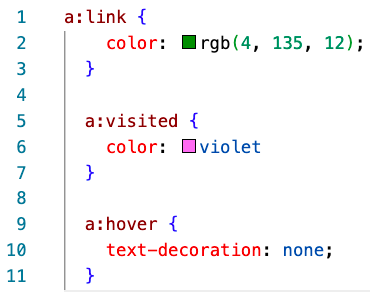
\includegraphics[height=0.4\paperheight]{fig/aula2/css_estado.png} \\
	  \end{center}
 \tiny Fontes: \cite{mdn2023}
\end{frame}

%-----------------------------------------------------
\section{Função CSS}
\begin{frame}{CSS Função}
Uma função consiste em chamar o nome de uma uma função e um par de perenteses, entre os parenteses são iformados os parâmetros.\\
No caso da função \textbf{calc()} o desenvolvedor inform que a largura da div deve ser 90\% do bloco onde ela está, menos 30px.\\
\begin{columns}
\begin{column}{0.5\textwidth}
        \begin{center}
		  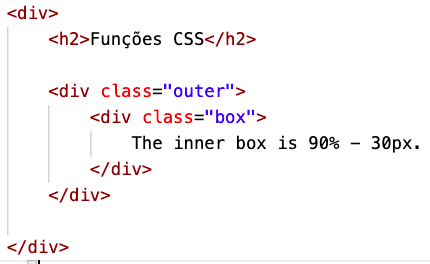
\includegraphics[height=0.4\paperheight]{fig/aula2/layout_html1.png} \\
		  \tiny{Código HTML}
	  \end{center}
   \end{column}
   \begin{column}{0.5\textwidth}
        \begin{center}
		  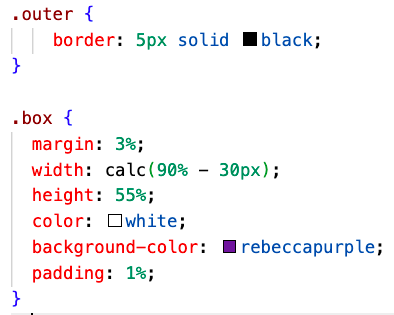
\includegraphics[height=0.4\paperheight]{fig/aula2/layout_css2.png} \\
		  \tiny{Código CSS}
	  \end{center}
	  
   \end{column}
\end{columns}
 \tiny Fontes: \cite{mdn2023}
\end{frame}
%-----------------------------------------------------
\begin{frame}{CSS Função}
Outro exemplo de função é a rotate aplicada a propriedade transform.\\
\begin{columns}
\begin{column}{0.5\textwidth}
        \begin{center}
		  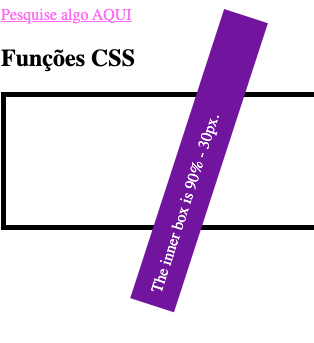
\includegraphics[height=0.4\paperheight]{fig/aula2/layout_html2.png} \\
		  \tiny{Saída do Código HTML}
	  \end{center}
   \end{column}
   \begin{column}{0.5\textwidth}
        \begin{center}
		  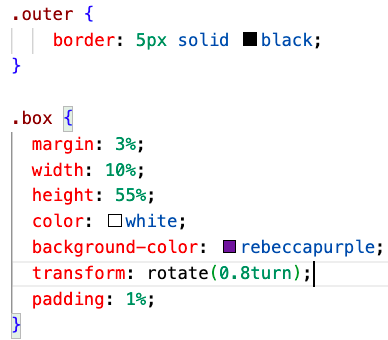
\includegraphics[height=0.4\paperheight]{fig/aula2/layout_css1.png} \\
		  \tiny{Código CSS: Edite o código anterior para width: 20\% e acrescente a propriedade transform.}
	  \end{center}
	  
   \end{column}
\end{columns}
 \tiny Fontes: \cite{mdn2023}
\end{frame}

%-----------------------------------------------------
\section{CSS Regras}
\begin{frame}{CSS Regras}
Regras CSS são aplicadas com o operador \@. E descrevem formatações CSS que só serão aplicadas dependendo de uma determinada condição.
\begin{columns}
\begin{column}{0.5\textwidth}
        A regra ao lado será aplicada apenas se o monitor que exibe o seu site tiver mais de 30em
   \end{column}
   \begin{column}{0.5\textwidth}
        \begin{center}
		  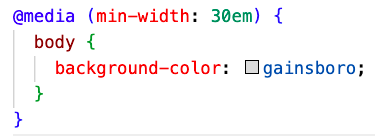
\includegraphics[height=0.2\paperheight]{fig/aula2/layout_css3.png} \\
		  \tiny{Código CSS: Acrescente este código ao CSS anterior.}
	  \end{center}
	  
   \end{column}
\end{columns}
Teste a visualização no modo celular nas opções de "inspecionar" do Chrome.\\
 \tiny Fontes: \cite{mdn2023}
\end{frame}

%-----------------------------------------------------
\section{Atividades}
\begin{frame}{Atividade 1}
Sobre barras de navegação. Vamos utilizar alguns conceitos conhecidos para criar uma barra de navegação 
vertical.
	\begin{center}
		  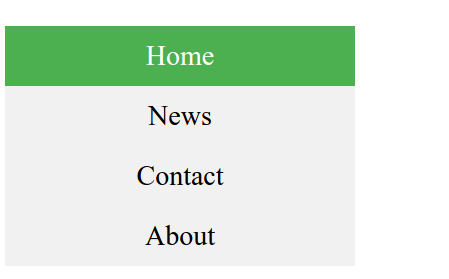
\includegraphics[height=0.4\paperheight]{fig/aula2/aep_1_2.png} \\
	  \end{center}
\end{frame}
%-----------------------------------------------------

\section{Referências}

\begin{frame}{Referências}%[allowframebreaks]
\small
\begin{center}
\tiny
\bibliographystyle{apalike}
\bibliography{ref_aula}
\end{center}
\end{frame}

\end{document}

\end{document}